% !TEX TS-program = pdflatex
% !TEX encoding = UTF-8 Unicode

% This is a simple template for a LaTeX document using the "article" class.
% See "book", "report", "letter" for other types of document.

\documentclass[12pt]{report} % use larger type; default would be 10pt

\usepackage[utf8]{inputenc} % set input encoding (not needed with XeLaTeX)

%%% Examples of Article customizations
% These packages are optional, depending whether you want the features they provide.
% See the LaTeX Companion or other references for full information.

%%% PAGE DIMENSIONS
\usepackage{geometry} % to change the page dimensions
\geometry{a4paper} % or letterpaper (US) or a5paper or....
% \geometry{margin=2in} % for example, change the margins to 2 inches all round
% \geometry{landscape} % set up the page for landscape
%   read geometry.pdf for detailed page layout information

\usepackage{graphicx} % support the \includegraphics command and options

% \usepackage[parfill]{parskip} % Activate to begin paragraphs with an empty line rather than an indent

%%% PACKAGES
\usepackage{booktabs} % for much better looking tables
\usepackage{array} % for better arrays (eg matrices) in maths
\usepackage{paralist} % very flexible & customisable lists (eg. enumerate/itemize, etc.)
\usepackage{verbatim} % adds environment for commenting out blocks of text & for better verbatim
\usepackage{subfig} % make it possible to include more than one captioned figure/table in a single float
% These packages are all incorporated in the memoir class to one degree or another...

%%% HEADERS & FOOTERS
\usepackage{fancyhdr} % This should be set AFTER setting up the page geometry
\pagestyle{fancy} % options: empty , plain , fancy
\renewcommand{\headrulewidth}{0pt} % customise the layout...
\lhead{}\chead{}\rhead{}
\lfoot{}\cfoot{\thepage}\rfoot{}

%%% SECTION TITLE APPEARANCE
\usepackage{sectsty}
\allsectionsfont{\sffamily\mdseries\upshape} % (See the fntguide.pdf for font help)
% (This matches ConTeXt defaults)

%%% RULE

\newcommand{\HRule}{\rule{\linewidth}{0.5mm}}

%%% BIBLIOGRAPHY

\usepackage{apacite}                           %bibliography in apa-style

%%% ToC (table of contents) APPEARANCE
\usepackage[nottoc,notlof,notlot]{tocbibind} % Put the bibliography in the ToC
\usepackage[titles,subfigure]{tocloft} % Alter the style of the Table of Contents
\renewcommand{\cftsecfont}{\rmfamily\mdseries\upshape}
\renewcommand{\cftsecpagefont}{\rmfamily\mdseries\upshape} % No bold!

\setcounter{secnumdepth}{-2}

%%% END Article customizations

%%% The "real" document content comes below...

\begin{document}

\begin{titlepage}

\begin{center}


% Upper part of the page

\includegraphics[width=1\textwidth]{./logo}\\[1cm]    

\textsc{\Large Bachelor Thesis}\\[0.5cm]
\textsc{\Large {[}201000166{]}}\\[0.5cm]


% Title
\HRule \\[0.4cm]
{ \huge \bfseries Research Proposal}\\[0.4cm]

\HRule \\[1.5cm]

% Author and supervisor
\begin{minipage}{0.4\textwidth}
\begin{flushleft} \large
\emph{Author:}\\
Micha \textsc{van den Enk} \\
{[}s1004654{]} \\
\end{flushleft}
\end{minipage}
\begin{minipage}{0.4\textwidth}
\begin{flushright} \large
\emph{Supervisors:} \\
Dr. H. H. \textsc{Leemkuil} \\
Second \textsc{supervisor} \\
\end{flushright}
\end{minipage}

\vfill

% Bottom of the page
{\large DATE}

\end{center}

\end{titlepage}

\tableofcontents

\chapter{Preface}

In this document the reader can find a proposal for designing a course on quantum mechanics in a qCraft learning environment. This is an assignment executed for a bachelor thesis. The document contains a table with general information, a short summary of the assignment, a detailed description of the assignment wth the rationale, the conceptual framework and the relevance, the design approach and a planning.

\chapter{General Information}

\begin{center}
\begin{tabular}{ l p{8cm} }
Researcher & Micha van den Enk (s1004654) \\
Study & Onderwijskunde \\
Study Department & Instructional Technology \\ 
Date & \\
First supervisor & Dr H. H. Leemkuil \\
Second supervisor & \\
Keywords & Quantum mechanics, Middle school Education, Netherlands \\
Title & \\
\end{tabular}
\end{center}

\chapter{Summary}

\chapter{Description}

\section{Rationale}

\section{Conceptual Framework}

\section{Relevance}

\chapter{Design approach}

A model which describes the process of developing educational resources is the Generic Model \cite{genericmodel} (see figure~\ref{fig:genmod}). It describes the phases Analysis, Design, Development, Implementation and Evaluation. This model will be partly used for this project. Because of time constraints and the limited size of the project it will only go as far as the horizontal bar of development, this will be elaborated further later in this chapter.

\begin{figure}[h]
\centering
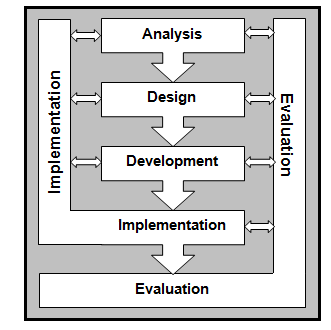
\includegraphics[width=0.7\textwidth]{genericmodel}
\caption{\footnotesize The generic model by \protect\citeA{genericmodel}\label{fig:genmod}}
\end{figure}

\section{Analyses}

The first step in the Generic Model \cite{genericmodel} is the step Analysis. In this step, data is gathered which is necessary for designing an effective solution. \citeA{smithragan} mention three different kinds of analysis, namely analyzing the learning context, analyzing the learners and analyzing the learning task.

\subsection{Analyzing the learning context}

A learning task always takes place in a certain learning context. In this case this is the middle school. It entails not only the place, but also the temporal and social environment \cite{smithragan}. The analysis of the learning context can provide the instructional needs and a description of the different factors influencing the instruction. With the instructional needs, the designer can establish the main learning goals for the instruction. The description of the learning environment can provide the learning opportunities and constraints which have to be taken into account for the instruction.

\subsection{Analyzing the learners}

The second analysis is that of the learners \cite{smithragan}. The purpose of this analysis is the characterization of the end user of the instruction, which is in this case the middle school students. For this analysis it is important to determine the similarities and differences between the learners. \citeA{smithragan} provide a list of factors which play a role in designing the instruction.

\subsection{Analyzing the learning task}

The final step is analyzing the learning task \cite{smithragan}. In this analysis the goals from the needs assessment during the analysis of the learning context have to be translated to test specifications, with which the content of the instruction can be established. In order to achieve these test specifications, first the type of learning has to be established. Having this established, the information-processing analysis can be conducted. Every type of learning has its own kind of information-processing analysis. When the information-processing analysis has been conducted, the next step is the prerequisite analysis. The outcome of this has to correspond to the outcome of the learner analysis. Finally, the learning objectives can be written, which form the test specifications. Every learning objective has to contain a description of the terminal behavior or actions that will demontsrate learning, a description of the conditions of demonstration of that action and a description of the standard or criterion \cite{smithragan}. Every learning objective will fall into a catagory of Bloom his taxanomy of learning objectives \cite{bloom}, and will use appropriate action verbs.

\section{Literature research}

After the analyses have been conducted, the literature research will take place. The first step of the literature research will be considering the search terms. For this, the results of the analyses will have to be taken into account, especially the characterizations of the learners and the learning task. The search terms will then be expanded by finding synonyms and similar relevant terms by using the Thesaurus. After the search terms are determined, it has to be established which databases will provide useful results. Then a cyclic process will take place in which the amount of results will be assessed with these databases and search terms and then if needed the results are limited or expanded by using more search terms and filters. The results will always be constrained to peer-reviewed articles. Other filters could than be the recency of the articles or the educational level of the test subjects.

When there is an appropriate amount of results, a literature matrix can be constructed. This matrix will contain research questions in the top row and the resulting articles in the left row. By using this technique, every question can be answered per resulting article. The columns can then be summarized in order to answer every question separately. These answers ultimately are the content of the theoretic framework.

\section{Design}

\section{Development}

\chapter{Planning}

\begin{center}
\begin{tabular}{ l r }
Analyses & 1 May \\
Literature research & 15 May \\
Design & 22 May \\
Development & 29 May \\
Evaluation & 12 June \\
Conclusion/Discussion & 19 June \\
Presentation & 26 June \\
\end{tabular}
\end{center}

\bibliographystyle{apacite}
\bibliography{references}

\end{document}
